\documentclass[journal]{IEEEtran}

%\usepackage[retainorgcmds]{IEEEtrantools}
%\usepackage{bibentry}
\usepackage{xcolor,soul,framed} %,caption

\colorlet{shadecolor}{yellow}
% \usepackage{color,soul}
\usepackage[pdftex]{graphicx}
\graphicspath{{../pdf/}{../jpeg/}}
\DeclareGraphicsExtensions{.pdf,.jpeg,.png}

\usepackage[cmex10]{amsmath}
%Mathabx do not work on ScribTex => Removed
%\usepackage{mathabx}
\usepackage{array}
\usepackage{mdwmath}
\usepackage{mdwtab}
\usepackage{eqparbox}
\usepackage{url}


% ----------------------------------------------

% Definitions of languages: ------------
\usepackage{listings}
\lstdefinestyle{cStyle}{
  basicstyle=\scriptsize,
  breakatwhitespace=false,
  breaklines=true,
  captionpos=b,
  keepspaces=true,
  numbersep=5pt,
  showspaces=false,
  gobble=4,
  tabsize=4,
  showstringspaces=false,
  showtabs=false,
}
\renewcommand*{\lstlistingname}{Code}

% ----------------------------------------------




% \hyphenation{op-tical net-works semi-conduc-tor}

%\bstctlcite{IEEE:BSTcontrol}


%=== TITLE & AUTHORS ====================================================================
\begin{document}
\bstctlcite{IEEEexample:BSTcontrol}
    \title{Imitation Learning with Keras}
  \author{Carlos~Matheus~Barros~da~Silva,~\IEEEmembership{Computer Engineering Bachelor Student of ITA}\\Prof. Marcos~Ricardo~Omena~de~Albuquerque~Máximo}

% The paper headers
\markboth{INSTITUTO TECNOLÓGICO DE AERONÁUTICA, May~2019
}{Neural Networks}

% ====================================================================
\maketitle



% === ABSTRACT ==============================================================
% ============================================================================
\begin{abstract}

This paper evaluates two Keras' Neural Network by test it in different scenarios with two simple tests and an imitation learning problem.

It was observed that the Neural Network worked fine for those purposes, and in some case, the result was really good, in the imitation learning case, for example.

% === KEYWORDS ===============================================================
% ============================================================================
\begin{IEEEkeywords}
    Simple Evolution Strategy, SES, Covariance Matrix Adaptation Evolution Strategy, CMA-ES, optimization
\end{IEEEkeywords}
\end{abstract}

\IEEEpeerreviewmaketitle

% ====================================================================
% ====================================================================
% ====================================================================


% === I. INTRODUCTION ========================================================
% =============================================================================
\section{Introduction}

\IEEEPARstart{N}{e}ural networks (NN) are computing systems vaguely inspired by the biological neural networks and astrocytes that constitute animal brains. The neural network itself is not an algorithm, but rather a framework for many different machine learning algorithms to work together and process complex data inputs. Such systems "learn" to perform tasks by considering examples, generally without being programmed with any task-specific rules. For example, an image recognition, they might learn to identify images that contain cats by analyzing example images that have been manually labeled as "cat" or "no cat" and using the results to identify cats in other images. They do this without any prior knowledge about cats, for example, that they have fur, tails, whiskers and cat-like faces. Instead, they automatically generate identifying characteristics from the learning material that they process.

Keras is an open-source neural-network library written in Python. It is capable of running on top of TensorFlow, Microsoft Cognitive Toolkit, Theano, or PlaidML. Designed to enable fast experimentation with deep neural networks, it focuses on being user-friendly, modular, and extensible. It was developed as part of the research effort of project ONEIROS (Open-ended Neuro-Electronic Intelligent Robot Operating System), and its primary author and maintainer is François Chollet, a Google engineer. Chollet also is the author of the XCeption deep neural network model.

In 2017, Google's TensorFlow team decided to support Keras in TensorFlow's core library. Chollet explained that Keras was conceived to be an interface rather than a standalone machine-learning framework. It offers a higher-level, more intuitive set of abstractions that make it easy to develop deep learning models regardless of the computational backend used. Microsoft added a CNTK backend to Keras as well, available as of CNTK v2.0.

Keras contains numerous implementations of commonly used neural-network building blocks such as layers, objectives, activation functions, optimizers, and a host of tools to make working with image and text data easier. The code is hosted on GitHub, and community support forums include the GitHub issues page and a Slack channel.

In addition to standard neural networks, Keras has support for convolutional and recurrent neural networks. It supports other common utility layers like dropout, batch normalization, and pooling.

Keras allows users to productize deep models on smartphones (iOS and Android), on the web, or on the Java Virtual Machine. It also allows the use of distributed training of deep-learning models on clusters of Graphics Processing Units (GPU) and Tensor processing units (TPU).

% ==========================================================================
\section{Neural Network Implementation}

The implementation was based on the file \textit{lenet5}. The essence of the implementation can be seen on the Code \ref{code:lenet}

\lstinputlisting[
    language=python,
    caption={Code of Convolutional Neural Network \textit{lenet5}},
    label={code:lenet},
    style=cStyle,
    firstline=5,
    lastline=83
]{./../code/imitation_learning.py}

\section{Neural Network Analysis}

\subsection{Keras' Neural Network Analysis without regularization}

In this analysis was used two test functions: \textit{sum greater than} and \textit{xor}. This initial analysis is not using regularization.

The Keras' Neural Network performed regular on \textit{sum greater than} function. On the graphs represented by the images from Image \ref{img:greater_cost_no_reg} to Image \ref{img:greater_classification_no_reg}. It is possible to verify that the result is overfitted on the Image \ref{img:greater_classification_no_reg} and the convergence is not so fast on the Image \ref{img:greater_cost_no_reg}.

\begin{figure}
  \begin{center}
  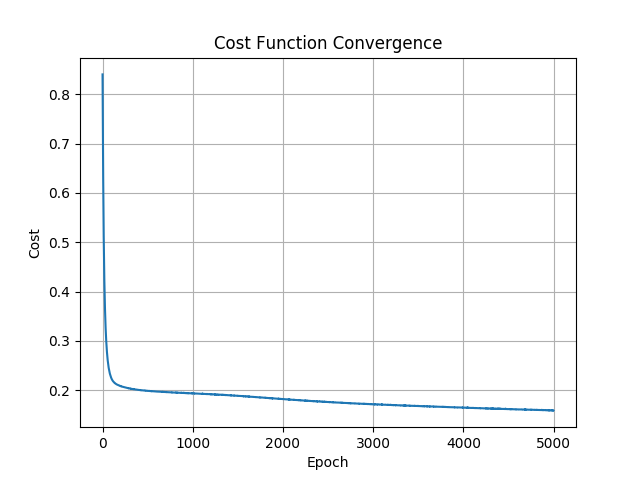
\includegraphics[width=2.8in]{./../code/sgz_result/convergence_sgz_l0_0.png}
  \caption{Convergence of cost function on greater than function test case, when it is not using regularization.}
  \label{img:greater_cost_no_reg}
  \end{center}
\end{figure}

\begin{figure}
  \begin{center}
  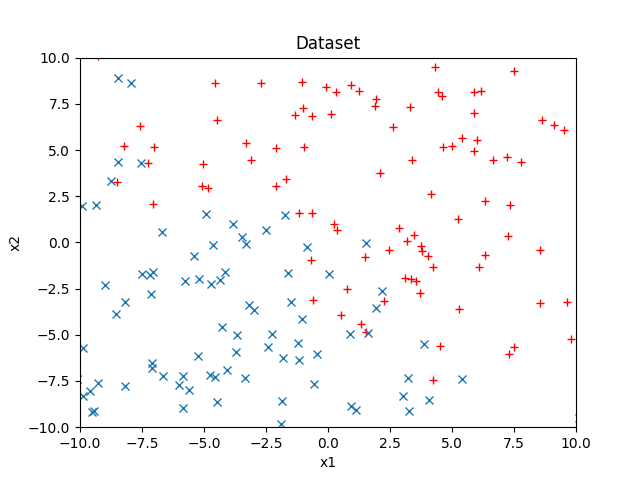
\includegraphics[width=2.8in]{./../code/sgz_result/dataset_sgz_l0_0.png}
  \caption{Dataset of greater than function.}
  \label{img:greater_data_set}
  \end{center}
\end{figure}

\begin{figure}
    \begin{center}
    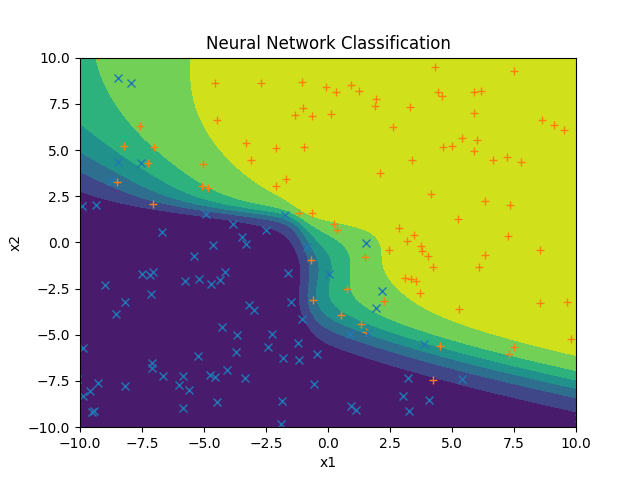
\includegraphics[width=2.8in]{./../code/sgz_result/nn_classification_sgz_l0_0.png}
    \caption{Neural Network Classification on greater than function, when it is not using regularization.}
    \label{img:greater_classification_no_reg}
    \end{center}
\end{figure}

The Neural Network performed regular on \textit{xor} function. On the graphs represented by the images from Image \ref{img:xor_cost_no_reg} to Image \ref{img:xor_classification_no_reg}. It is also possible to see that in this case, it also heaped some overfit causing some distortion and leading to some mistakes on the data set on the graph represented by the Image \ref{img:xor_classification_no_reg}.

\begin{figure}
  \begin{center}
  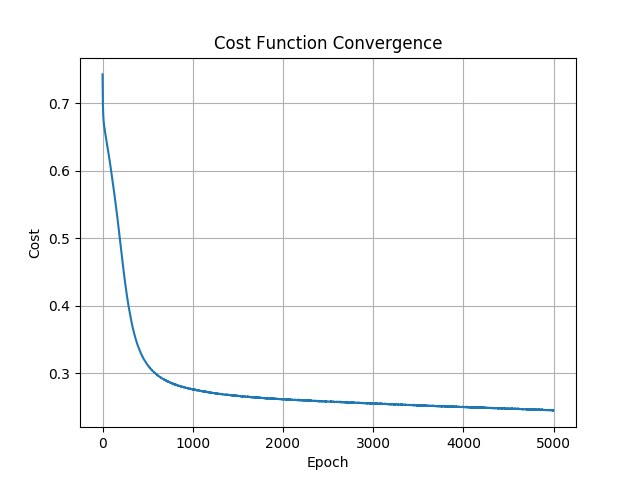
\includegraphics[width=2.8in]{./../code/xor_result/convergence_xor_l0_0.png}
  \caption{Convergence of cost function on xor function test case, when it is not using regularization.}
  \label{img:xor_cost_no_reg}
  \end{center}
\end{figure}

\begin{figure}
  \begin{center}
  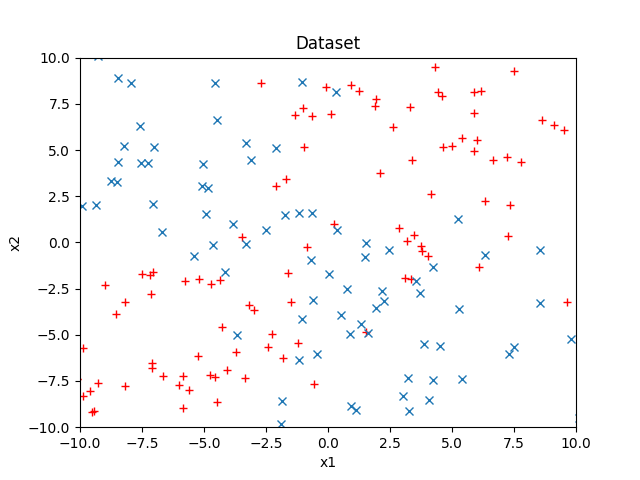
\includegraphics[width=2.8in]{./../code/xor_result/dataset_xor_l0_0.png}
  \caption{Dataset of xor function.}
  \label{img:xor_data_set}
  \end{center}
\end{figure}

\begin{figure}
    \begin{center}
    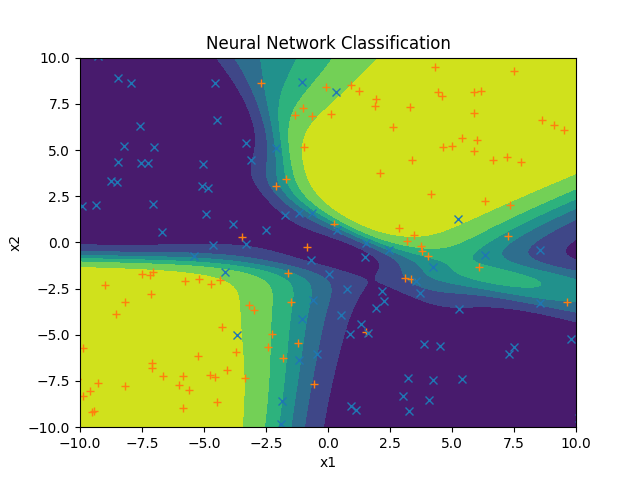
\includegraphics[width=2.8in]{./../code/xor_result/nn_classification_xor_l0_0.png}
    \caption{Neural Network Classification on xor function, when it is not using regularization.}
    \label{img:xor_classification_no_reg}
    \end{center}
\end{figure}

\subsection{Keras' Neural Network Analysis without regularization}

In this analysis was used the same two test functions: \textit{sum greater than} and \textit{xor}. But now using regularization $\lambda_{l_2} = 0.002$.

The Keras' Neural Network performed well on \textit{sum greater than} function. On the graphs represented by the images from Image \ref{img:greater_cost_reg} to Image \ref{img:greater_classification_reg}. It is possible to verify that the result now is much less overfitted on the Image \ref{img:greater_classification_reg}, it is much softer, and the convergence is now faster on the Image \ref{img:greater_cost_reg}.

\begin{figure}
  \begin{center}
  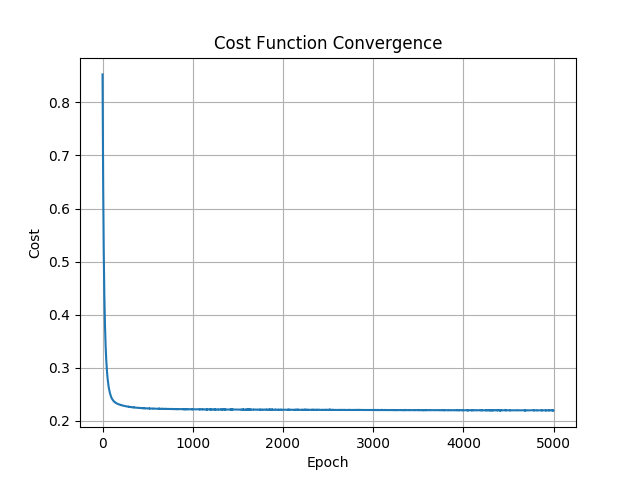
\includegraphics[width=2.8in]{./../code/sgz_result/convergence_sgz_l0_002.png}
  \caption{Convergence of cost function on greater than function test case, when it is using regularization.}
  \label{img:greater_cost_reg}
  \end{center}
\end{figure}

\begin{figure}
    \begin{center}
    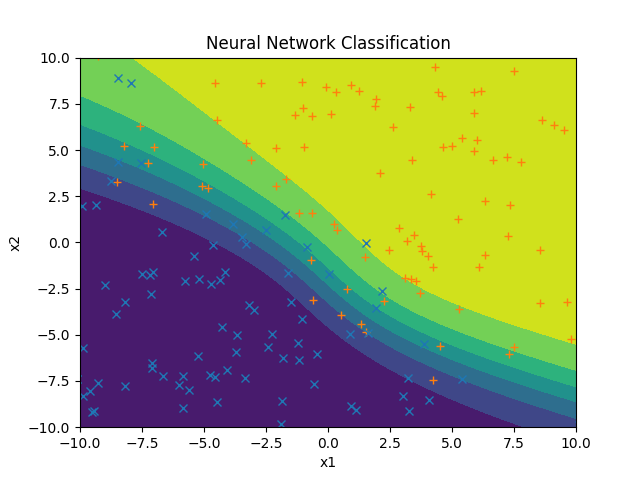
\includegraphics[width=2.8in]{./../code/sgz_result/nn_classification_sgz_l0_002.png}
    \caption{Neural Network Classification on greater than function, when it is using regularization.}
    \label{img:greater_classification_reg}
    \end{center}
\end{figure}

The Neural Network performed well on \textit{xor} function. On the graphs represented by the images from Image \ref{img:xor_cost_reg} to Image \ref{img:xor_classification_reg}. It is also possible to see that in this case, it also heaped much less overfit leading to a much softer image on the graph represented by the Image \ref{img:xor_classification_reg}.

\begin{figure}
  \begin{center}
  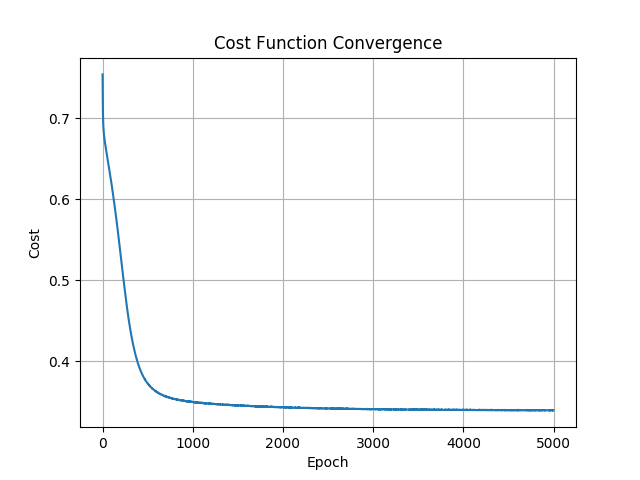
\includegraphics[width=2.8in]{./../code/xor_result/convergence_xor_l0_002.png}
  \caption{Convergence of cost function on xor function test case, when it is using regularization.}
  \label{img:xor_cost_reg}
  \end{center}
\end{figure}

\begin{figure}
    \begin{center}
    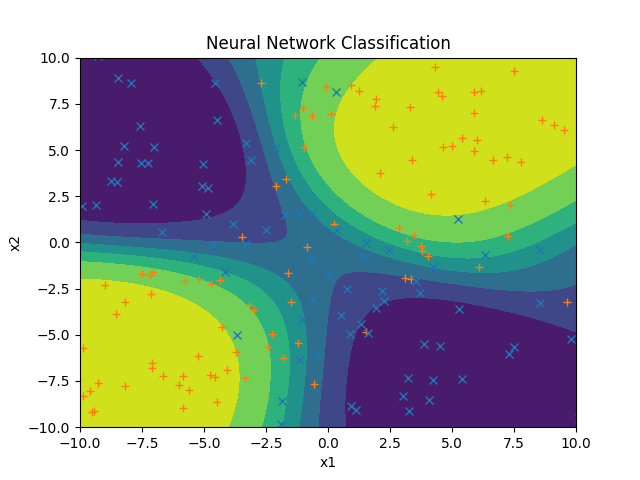
\includegraphics[width=2.8in]{./../code/xor_result/nn_classification_xor_l0_002.png}
    \caption{Neural Network Classification on xor function, when it is using regularization.}
    \label{img:xor_classification_reg}
    \end{center}
\end{figure}

\subsection{Keras' Neural Network Analysis in Imitation Learning}

In order to do the Imitation Learning, it was used the Code \ref{code:imitation} implementation.

It was made using Keras, not using regularization, and using mean squared error.

The result of this Neural Network on the robot movement can be seen on the graphs from Image \ref{img:right_ankle_pitch} to Image \ref{img:right_knee_pitch}.

\begin{figure}
  \begin{center}
  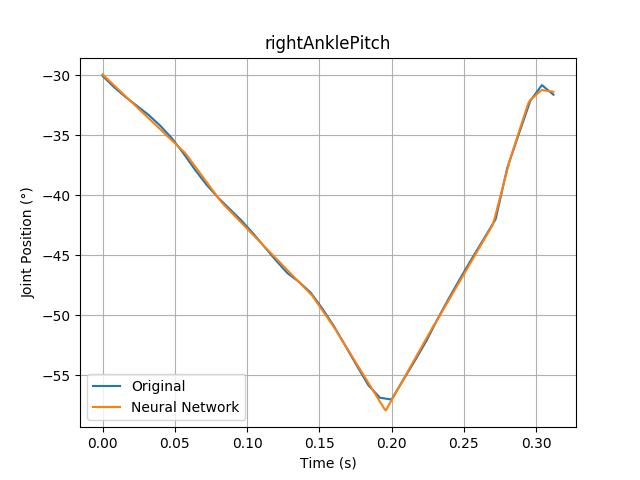
\includegraphics[width=2.8in]{./../code/imitation_learning_result/rightAnklePitch.png}
  \caption{Neural Network's movement imitation of robot's right ankle pitch}
  \label{img:right_ankle_pitch}
  \end{center}
\end{figure}

\begin{figure}
  \begin{center}
  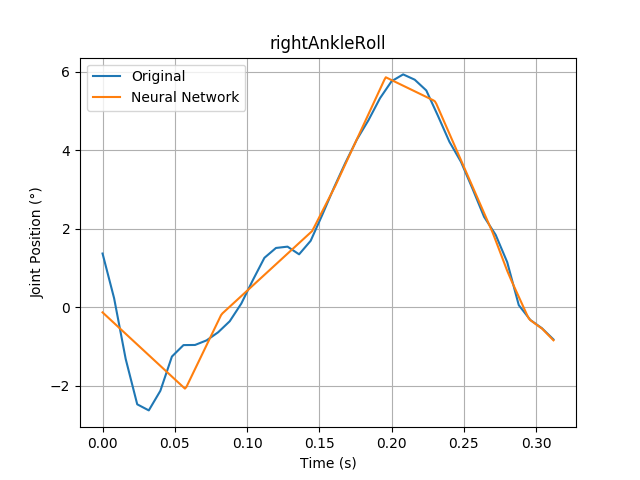
\includegraphics[width=2.8in]{./../code/imitation_learning_result/rightAnkleRoll.png}
  \caption{Neural Network's movement imitation of robot's right ankle roll}
  \label{img:right_ankle_roll}
  \end{center}
\end{figure}

\begin{figure}
  \begin{center}
  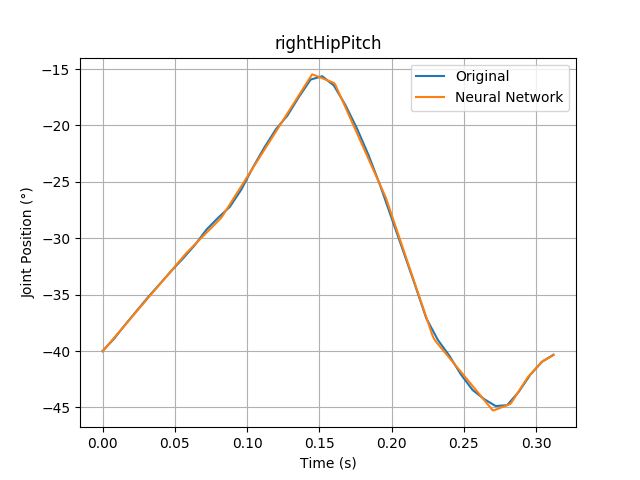
\includegraphics[width=2.8in]{./../code/imitation_learning_result/rightHipPitch.png}
  \caption{Neural Network's movement imitation of robot's right Hip pitch}
  \label{img:right_hip_pitch}
  \end{center}
\end{figure}

\begin{figure}
  \begin{center}
  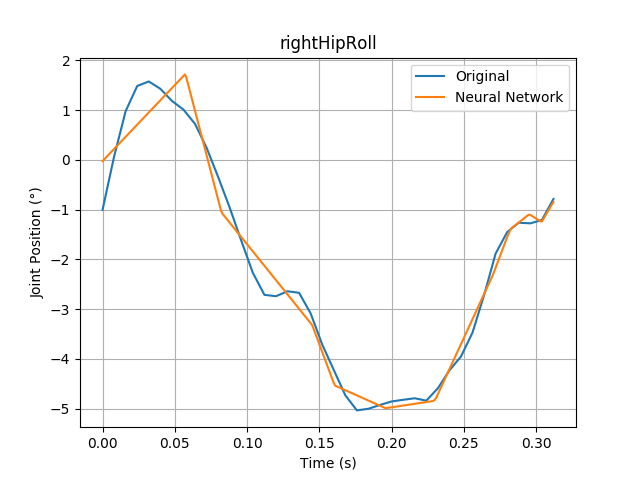
\includegraphics[width=2.8in]{./../code/imitation_learning_result/rightHipRoll.png}
  \caption{Neural Network's movement imitation of robot's right hip roll}
  \label{img:right_hip_roll}
  \end{center}
\end{figure}

\begin{figure}
  \begin{center}
  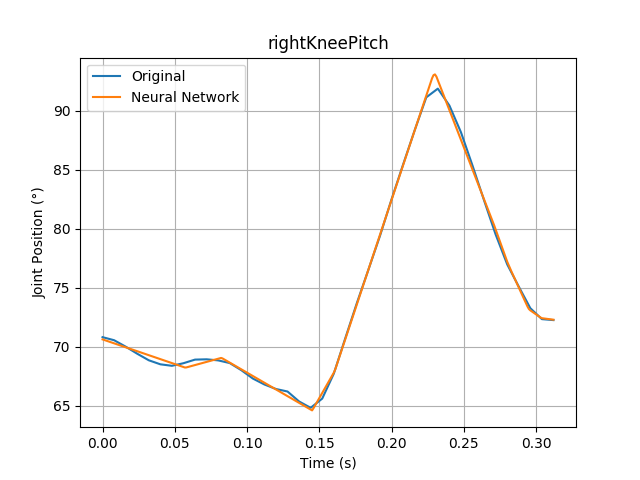
\includegraphics[width=2.8in]{./../code/imitation_learning_result/rightKneePitch.png}
  \caption{Neural Network's movement imitation of robot's right Knee pitch}
  \label{img:right_knee_pitch}
  \end{center}
\end{figure}

\section {Conclusion}

It was clear, therefore, that the Keras' Neural Network worked as expected. Both test cases (greater than function and xor function) the Neural Network worked as well, with a much better result with regularization, because without regularization the results were overfitted.

For the Imitation Learning with Keras, the results were good in some cases and very precise in most some cases.

\vfill
\end{document}
